\documentclass{article}
\usepackage[utf8]{inputenc}
\usepackage{setspace}
\usepackage{tikz}
\usetikzlibrary{positioning}
\usepackage{amsfonts}
\usepackage{amssymb}
\usepackage{amsmath}
\usepackage{amsthm}
\usepackage{systeme}
\usepackage{mathtools}
\usepackage{hyperref}
\usepackage{venndiagram}
\usepackage{pgfplots}
\usepgfplotslibrary{statistics}
\pgfplotsset{compat=1.18}

\begin{document}

\section*{Question 1}

~

\subsection*{a}

~

\begin{align*}
    &H_0:\mu=6\\
    &H_a:\mu>6\\
\end{align*}

~

\subsection*{b}

~

\begin{align*}
    &\text{Suppose that the null hypothesis is true, that the average height is 6 inches}\\
\end{align*}

~

\subsection*{c}

~

\begin{align*}
    &z=\frac{\overline{x}-\mu}{\frac{s}{\sqrt{n}}}\\
    &=\frac{\overline{x}-6}{\frac{}{\sqrt{72}}}\\
\end{align*}

~

\subsection*{d}

~

Significance level is 0.03

~

\subsection*{e}

~

\begin{align*}
    &\overline{x}=\mu+z_{0.03}(\frac{s}{\sqrt{n}})\\
    &=6+1.88(\frac{1}{\sqrt{72}})\\
    &=6.22\\
\end{align*}

~

\subsection*{f}

~

\begin{align*}
    &\mu=6.5\\
    &\text{type 2 error}\\
    &\beta=P(\overline{x}<6.22)\\
    &=P(\frac{\overline{x}-\mu}{\frac{s}{\sqrt{n}}}<\frac{6.22-6.5}{\frac{1}{\sqrt{72}}})\\
    &=P(z<-2.38)\\
    &=0.0086\\
    &\text{Power of test}1:-\beta=1-0.0086=0.9914\\
\end{align*}
\newpage

\section*{Question 3}

~

\subsection*{a}

~

\begin{align*}
    &\text{Median}=\frac{1.78+1.83}{2}=1.805\\
    &Q_1=\frac{1.67+1.70}{2}=1.685\\
    &Q_3=\frac{1.91+2.00}{2}=1.955\\
    &IQR=Q_3-Q_1=0.27\\
    &\text{upper bound}=Q_3+1.5IQR=2.36\\
    &\text{lower bound}=Q_1-1.5IQR=1.28\\
    &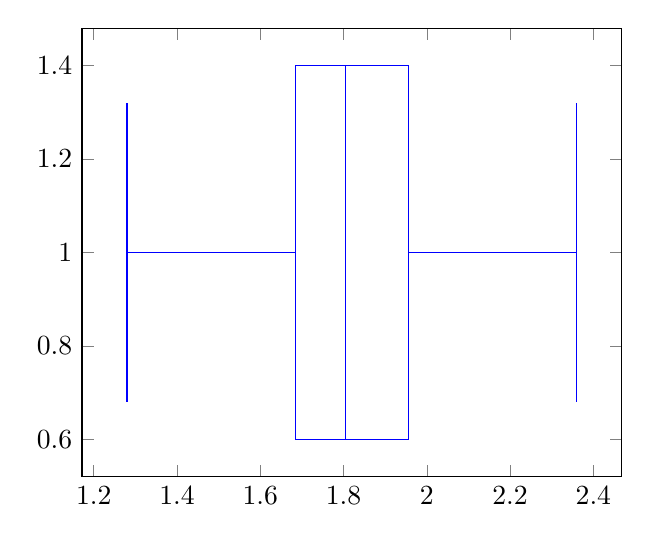
\begin{tikzpicture}
        \begin{axis}
            \addplot+[
            boxplot prepared={
            median=1.805,
            upper quartile=1.955,
            lower quartile=1.685,
            upper whisker=2.36,
            lower whisker=1.28
          },
          ] coordinates {};
        \end{axis}
      \end{tikzpicture}\\
\end{align*}

~

The boxplot shows there are no outliers, and there the samples are symmetry, suggesting that the distribution is normal and centered around 1.8.

~

\subsection*{b}

~

\begin{align*}
    &H_0:\mu=1.5\\
    &H_a:\mu\ne1.5\\
    &t=\frac{\overline{x}-\mu}{\sigma/\sqrt{n}}\\
    &=\frac{1.81625-1.5}{0.2105/\sqrt{8}}\\
    &=4.249\\
    &t_{a/2,n-1}=2.365\\
    \Rightarrow&t>t_{a/2,n-1}\\
    &\text{The null hypothesis is rejected}\\
\end{align*}

~

\subsection*{c}

~

Q-Q plot of the eight samples shows that the distribution is roughly normal, so the normality assumption is justified and t test is applicable.

\newpage

\section*{Question 4}

~

\subsection*{a}

~

\begin{align*}
    &\hat{p}=\frac{14}{100}=0.14\\
    &p_0=0.1\\
    &H_0:p=0.1\\
    &H_a:p>0.1\\
    &z=\frac{\hat{p}-p_0}{\sqrt{\frac{p_0(1-p_0)}{100}}}\\
    &=\frac{0.14-0.1}{\sqrt{\frac{0.1\times0.9}{100}}}\\
    &=\frac{0.04}{0.03}\\
    &=1.33\\
    &P=P[Z>z]\\
    &=1-P[Z<1.33]\\
    &=1-0.9082\\
    &=0.0918>0.05\\
    &\text{fail,type 2 error: fail to reject the null hypothesis}\\
\end{align*}

~

\subsection*{b}

~

\begin{align*}
    &p'=0.15\\
    &\\
    &n=100:\\
    &\beta(p')=\Phi\left[\frac{p_0-p'+z_{0.05}\sqrt{\frac{p_0(1-p_0)}{n}}}{\sqrt{\frac{p'(1-p')}{n}}}\right]\\
    &=\Phi\left[\frac{0.1-0.15+1.645\sqrt{\frac{0.1(1-0.1)}{100}}}{\sqrt{\frac{0.15(1-0.15)}{100}}}\right]\\
    &=\Phi[-0.0182]\\
    &=0.4927\\
    &\\
    &n=200:\\
    &\beta(p')=\Phi\left[\frac{p_0-p'+z_{0.05}\sqrt{\frac{p_0(1-p_0)}{n}}}{\sqrt{\frac{p'(1-p')}{n}}}\right]\\
    &=\Phi\left[\frac{0.1-0.15+1.645\sqrt{\frac{0.1(1-0.1)}{200}}}{\sqrt{\frac{0.15(1-0.15)}{200}}}\right]\\
    &=\Phi[-0.5982]\\
    &=0.2749\\
\end{align*}

~

\subsection*{c}

~

\begin{align*}
    &n=(\frac{z_{0.05}\sqrt{0.1(1-0.1)}+z_{0.1}\sqrt{0.15(1-0.15)}}{0.15-0.1})^2\\
    &=(\frac{1.645\sqrt{0.1(1-0.1)}+1.28\sqrt{0.15(1-0.15)}}{0.15-0.1})^2\\
    &=361.419\\
    &\approx362\\
\end{align*}

\newpage

\section*{Collaborators}

~

Frank Zhu

~

Jeffery Shu

~

Sam Sun


\end{document}